\chapter{可对易可观测量、能量相位与自旋进动}

\lectureoverview{我们从不确定性的定性含义开始。两个可观测量只有在拥有一组完备的共同本征基时才能同时具有确定值，而这等价于它们的算符对易。随后我们回顾幺正演化与Schr\"odinger方程，将交换子与经典泊松括号作比较，在能量基下求解含时方程，并把结果应用于磁场中的自旋。最后的计算给出自旋期望值的进动、一般自旋哈密顿量的两个能级，以及横向期望值与半个能隙能量的光子之间的区别。}

二态自旋仍然是我们最简单的量子系统。三态希尔伯特空间将是下一个最简单的抽象可能性；两个自旋已经具有四个正交基态。我们暂时还不组合两个自旋，尽管这一步已经不远，并且会随之带来纠缠。首先我们应当完成单自旋问题，并把不确定性与时间演化的观念建立在更牢固的基础上。

\section{当两个量能够同时具有确定值时}

好的测量是可重复的。如果测量一个可观测量并得到值\(l\)，那么立即重复测量应当返回同一个值。因此，第一次测量必须使系统——至少暂时地——处于相应算符的一个本征态：
\begin{equation}
L\ket{l}=l\ket{l}.
\end{equation}
这一操作性的陈述已足以揭示不确定性的定性起源。

假设两个可观测量\(L\)与\(M\)能够被同时测量。联合测量必须使两个报告值都保持确定。因此，其可能的测量后状态必须是两个算符的共同本征向量。在这里所用的有限维情形中，我们可以选取一组完备正交归一集\(\{\ket{i}\}\)，满足
\begin{equation}
L\ket{i}=l_i\ket{i},
\qquad
M\ket{i}=m_i\ket{i}.
\label{eq:l5-common-eigenvectors}
\end{equation}

\begin{remark}
\emph{基}一词将指完备正交归一基。线性代数允许非正交基，但正交归一约定对量子态尤为自然。简并本征值会在一个本征空间内留下自由度；在该空间内，本征向量可以选为正交归一的。
\end{remark}

\begin{theorem}
两个有限维厄米可观测量能够被同时测量，当且仅当它们容许一组完备的共同本征基，等价地，当且仅当它们对易。
\end{theorem}

正向由式~\eqref{eq:l5-common-eigenvectors}立即可得。按一种顺序作用给出
\begin{align}
ML\ket{i}
&=M\bigl(l_i\ket{i}\bigr)\\
&=l_i m_i\ket{i},
\end{align}
而按相反顺序作用给出
\begin{align}
LM\ket{i}
&=L\bigl(m_i\ket{i}\bigr)\\
&=m_i l_i\ket{i}.
\end{align}
本征值是普通数，所以\(l_i m_i=m_i l_i\)。因此\(ML\)与\(LM\)对基的每个成员作用相同，从而对每个态作用相同：
\begin{equation}
[L,M]\equiv LM-ML=0.
\label{eq:l5-commuting-condition}
\end{equation}

\begin{figure}[htbp]
\centering
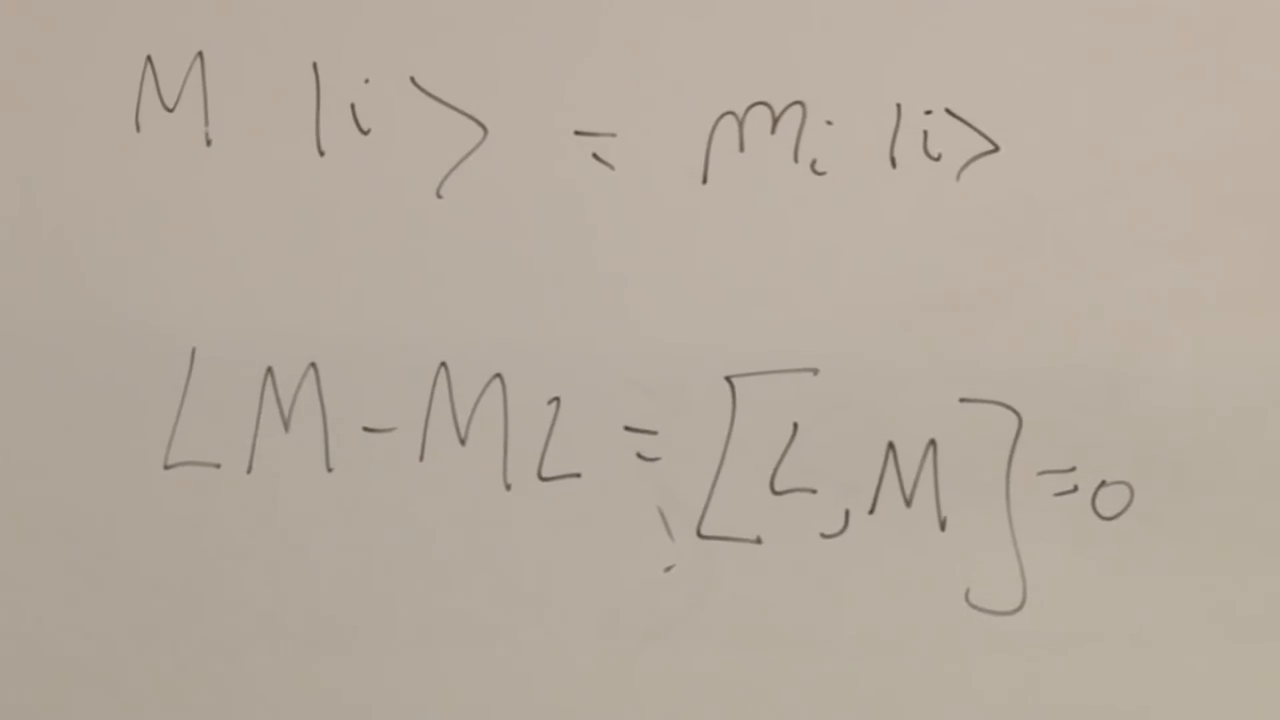
\includegraphics[width=0.86\textwidth]{lecture_05_figure_02.png}
\caption{共同本征向量的论证得到\(LM-ML=[L,M]=0\)。}
\lectureframe{00:10:30}
\end{figure}

逆命题也成立：对易的厄米算符可以被同时对角化。如果一个算符具有简并本征空间，另一个算符保持该本征空间不变，并且可以在其中被对角化。在每个本征空间中重复这一做法，便产生一组完备的共同本征基。

泡利算符给出第一个重要的反例。\(\sigma_x,\sigma_y,\sigma_z\)中没有两个对易。\(\sigma_z\)的本征态是上旋与下旋，而\(\sigma_x\)的本征态是右旋与左旋。人们可以制备其中一个分量的确定值并重复其测量，但不能同时制备两个分量的确定值。这就是在引入任何数值不等式之前的不确定性。

稍后我们将定量说明两个不对易可观测量的不确定性如何相互制约。这里并未证明任何数值不确定性原理。当前要点先于该不等式：不对易性阻止一个态同时给两个量赋予确定值。

\begin{classroomqa}
\audiencequestion{为什么同时测量要求共同本征向量？}
\lecturerresponse{可重复的测量使一个态具有确定的被测值，这意味着它是被测算符的一个本征态。如果两个值被一起得到并且都保持可重复，那么所得状态必须是两个算符的本征态。因此，联合结果的完备集合提供了一组共同本征基。}
\end{classroomqa}

\begin{classroomqa}
\audiencequestion{这涉及两个不同的粒子吗？}
\lecturerresponse{不一定，因为\(\sigma_x\)与\(\sigma_z\)已经作用于一个自旋。然而，对于两个不同的子系统，作用于不同因子的可观测量确实对易：\(A\otimes I\)与\(I\otimes B\)对易。这就是为什么一个自旋的一个分量与另一个自旋的一个分量能够被一起测量。组合这样的系统稍后将导致纠缠。}
\end{classroomqa}

\section{幺正演化及其生成元}

量子力学在定义状态上比经典力学花了长得多的时间，但一旦确立了状态空间，运动规则就很紧凑。设
\begin{equation}
\ket{\psi(t)}=U(t)\ket{\psi(0)}.
\label{eq:l5-propagator}
\end{equation}
时间演化必须保持可区分性。更强地说，它保持所有内积。对于一组正交归一基，
\begin{equation}
\bra{j}U^\dagger(t)U(t)\ket{i}=\delta_{ji},
\end{equation}
因此
\begin{equation}
U^\dagger(t)U(t)=I.
\label{eq:l5-unitarity}
\end{equation}
演化算符是幺正的。

在零经过时间时\(U(0)=I\)。连续性随后表明，经过小时间\(\epsilon\)的演化与恒等算符仅略有不同。在\(\hbar=1\)的单位制下，写为
\begin{equation}
U(\epsilon)=I-i\epsilon H+O(\epsilon^2),
\qquad
U^\dagger(\epsilon)=I+i\epsilon H^\dagger+O(\epsilon^2).
\end{equation}
代入方程~\eqref{eq:l5-unitarity}得到
\begin{equation}
H^\dagger=H.
\end{equation}
时间演化的生成元是厄米的，因此是一个可观测量。它就是哈密顿量。

将无穷小传播子作用于一个状态得到
\begin{equation}
\ket{\psi(\epsilon)}
=\ket{\psi(0)}-i\epsilon H\ket{\psi(0)}+O(\epsilon^2).
\end{equation}
重新整理得到黑板上展示的差商：
\begin{equation}
\frac{\ket{\psi(\epsilon)}-\ket{\psi(0)}}{\epsilon}
=-iH\ket{\psi(0)}+O(\epsilon).
\end{equation}

\begin{figure}[htbp]
\centering
\includegraphics[width=0.86\textwidth]{lecture_05_figure_03.png}
\caption{写成差商的无穷小更新。}
\lectureframe{00:23:33}
\end{figure}

取\(\epsilon\to0\)得到含时Schr\"odinger方程：
\begin{equation}
\frac{d}{dt}\ket{\psi(t)}=-iH\ket{\psi(t)}.
\label{eq:l5-schrodinger}
\end{equation}
恢复常数后，这就是\(i\hbar\,d\ket{\psi}/dt=H\ket{\psi}\)。

Schr\"odinger最初的方程涉及运动粒子的波函数。上述算符陈述曾被称为广义Schr\"odinger方程，因为它同样适用于自旋、三态系统、两个自旋或任意复杂度的系统。这个形容词已基本被弃用；现在这简单地就是该方程的一般形式。

方程~\eqref{eq:l5-schrodinger}给出了系统不受扰动时状态的确定演化。这并不使每个实验结果都确定。量子态决定可能测量的概率，而该方程通过变化的振幅更新这些概率。测量通常会改变状态并中断这种孤立演化。

\begin{classroomqa}
\audiencequestion{每次测量都会扰动系统吗？}
\lecturerresponse{一般来说，是的，但有一个重要的特例。如果状态已经是该可观测量的本征态，理想的重复测量可以确认其值而不改变该状态。一般而言失效的是，在不扰动其他不相容性质的情况下测量任意可观测量的可能性。}
\end{classroomqa}

\section{能量与定态方程}

因为\(H\)是厄米的，其特征值是实数，其特征向量可以选为完备正交归一基：
\begin{equation}
H\ket{E_i}=E_i\ket{E_i}.
\label{eq:l5-time-independent}
\end{equation}
这是Schr\"odinger方程的定态形式。它是一个本征值问题而非运动方程：它询问系统可以具有哪些能量值，以及哪些状态具有这些确定值。

谱取决于系统。束缚原子运动和谐振子具有可数的能级。非束缚粒子可能具有连续谱。能量可以通过许多方式测量；原则上，即使足够精确的质量测量也可以利用\(E=mc^2\)，尽管这很少是实用方法。真实系统已经具有其哈密顿量；物理学家并不规定它，而是试图发现它。一旦该算符已知，找出其特征值和特征向量就是数学任务。

向\(H\)加上常数\(cI\)会使每个能量移动\(c\)。它将整个状态乘以一个共同的相位\(e^{-ict}\)，这不改变概率或期望值。只有能量差影响此处考虑的动力学。

\section{期望值如何变化}

标准短语\emph{期望值}意指统计平均。对于可观测量\(L\)，
\begin{equation}
\expect{L}(t)=\bra{\psi(t)}L\ket{\psi(t)}.
\end{equation}
在此阶段只有态矢量携带时间依赖性。对两边求导并利用方程~\eqref{eq:l5-schrodinger}及其厄米共轭，
\begin{equation}
\frac{d}{dt}\ket{\psi}=-iH\ket{\psi},
\qquad
\frac{d}{dt}\bra{\psi}=i\bra{\psi}H,
\end{equation}
得到
\begin{align}
\frac{d}{dt}\expect{L}
&=i\bra{\psi}HL\ket{\psi}
  -i\bra{\psi}LH\ket{\psi}\\
&=-i\expect{[L,H]}.
\label{eq:l5-expectation-motion}
\end{align}

\begin{figure}[htbp]
\centering
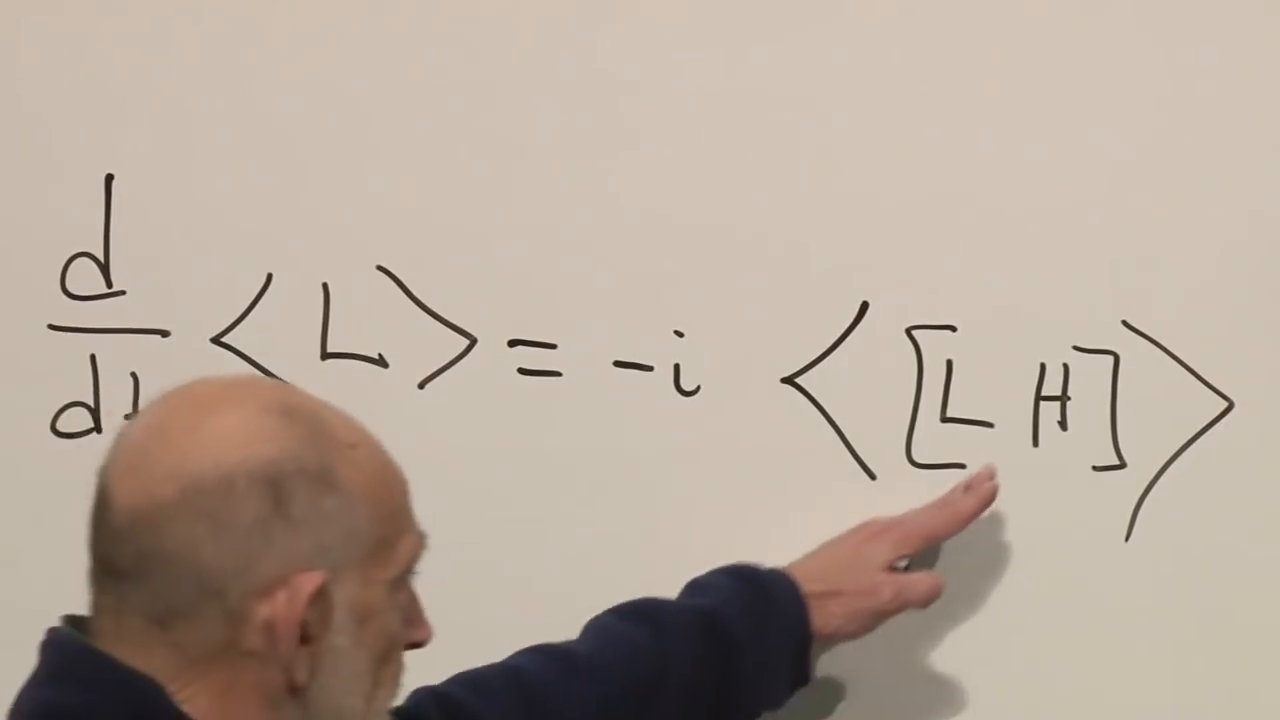
\includegraphics[width=0.86\textwidth]{lecture_05_figure_04.png}
\caption{对易子形式的期望值运动方程。}
\lectureframe{00:35:35}
\end{figure}

因子\(i\)并不威胁\(\expect{L}\)的实在性。对于厄米\(L\)和\(H\)，对易子是反厄米的：
\begin{equation}
[L,H]^\dagger=-[L,H].
\end{equation}
因此其期望值纯为虚数，所以乘以\(-i\)给出实数导数。

人们有时写下简写
\begin{equation}
\dot L=-i[L,H].
\end{equation}
此时它应被理解为方程~\eqref{eq:l5-expectation-motion}的缩写，一个关于平均值的方程。算符本身携带时间依赖性的完整图像变换将在后面出现。

\subsection{对易子的代数}

对易子是反对称的：
\begin{equation}
[A,B]=-[B,A].
\end{equation}
它们还满足一个与导数莱布尼茨法则类似乘积法则：
\begin{equation}
[AB,C]=A[B,C]+[A,C]B.
\label{eq:l5-product-rule}
\end{equation}
要验证它，保持每个因子的顺序：
\begin{align}
A[B,C]+[A,C]B
&=A(BC-CB)\\
&\quad +(AC-CA)B\\
&=ABC-ACB\\
&\quad +ACB-CAB\\
&=ABC-CAB\\
&=[AB,C].
\end{align}

\begin{figure}[htbp]
\centering
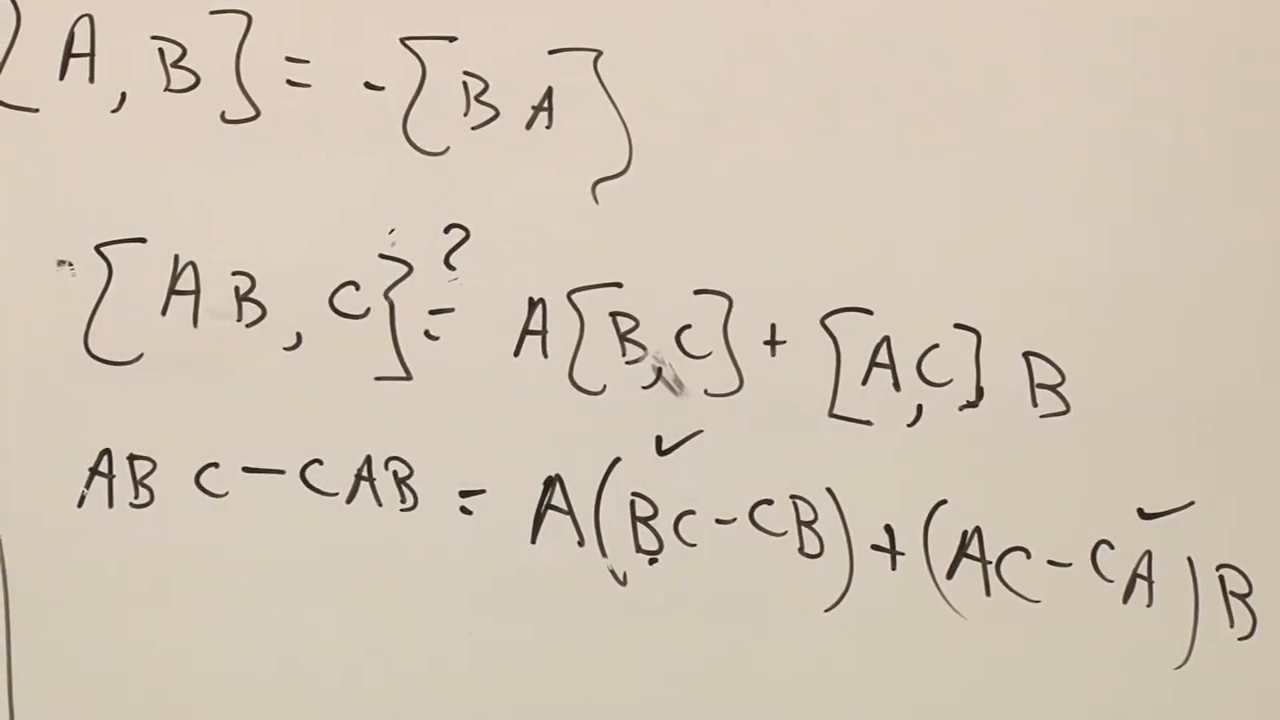
\includegraphics[width=0.86\textwidth]{lecture_05_figure_05.png}
\caption{通过展开两边验证的对易子乘积法则。}
\lectureframe{00:43:10}
\end{figure}

\begin{classroomqa}
\audiencequestion{乘积法则的右边是否意外地把左边计算了两次？}
\lecturerresponse{不会。展开时，\(ABC\)和\(-CAB\)正是所期望的两项。插入的两项是\(-ACB\)和\(+ACB\)，它们恰好相消。表面上多出的那一份，是为了以两种所需方式分解表达式而暂时需要的项。}
\end{classroomqa}

同样的反对称性和乘积法则对经典泊松括号也成立。这种结构上的相似并非偶然。经典对应关系是
\begin{equation}
\{A,B\}
\quad\longleftrightarrow\quad
\frac{1}{i\hbar}[A,B]
=-\frac{i}{\hbar}[A,B].
\label{eq:l5-poisson-correspondence}
\end{equation}
在\(\hbar=1\)单位下，经典方程
\begin{equation}
\frac{dL}{dt}=\{L,H\}
\end{equation}
与方程~\eqref{eq:l5-expectation-motion}具有相同的形式。在通常的宏观单位下，\(\hbar\)极小，对易子在适当的经典极限下变得可以忽略。这是把量子生成元\(H\)与经典力学的哈密顿量等同起来的关键检验。

\(\hbar\)这个因子在量纲上是必需的。泊松括号对共轭坐标和动量求导，而算符对易子则直接由乘积构成。普朗克常数提供了这些量纲之间的换算。

令\(L=H\)。由于每个算符都与自身对易，
\begin{equation}
\frac{d}{dt}\expect{H}
=-i\expect{[H,H]}=0.
\end{equation}
对于所讨论的与时间无关的哈密顿量，平均能量守恒。关于完整的能量分布还可以有更强的陈述，但这里只需要平均值。

\begin{classroomqa}
\audiencequestion{这些方程中的\(L\)是什么？它是角动量吗？}
\lecturerresponse{这里\(L\)是一个一般的厄米线性算符，因此是任意可观测量。它可以是自旋分量、位置，甚至\(H\)本身。这个字母取自\emph{线性算符}，除非另有说明，不应读作角动量。}
\end{classroomqa}

\begin{classroomqa}
\audiencequestion{为什么因子\(i\)不会使实的平均值产生虚的导数？}
\lecturerresponse{两个厄米算符的对易子是反厄米的，因此其期望值是虚的。下面的泡利矩阵计算使这一点具体化：它们的对易子含有显式的因子\(2i\)，它抵消了运动方程中的\(-i\)。}
\end{classroomqa}

\section{在能量基中求解Schr\"odinger方程}

假设能量本征值问题已经解出。将任意态在固定的能量基中展开：
\begin{equation}
\ket{\psi(t)}=\sum_j\alpha_j(t)\ket{E_j}.
\label{eq:l5-energy-expansion}
\end{equation}
在这个描述中基矢量不变；所有时间依赖性都在系数中。将方程~\eqref{eq:l5-energy-expansion}代入方程~\eqref{eq:l5-schrodinger}得到
\begin{align}
\sum_j\dot\alpha_j(t)\ket{E_j}
&=-i\sum_j\alpha_j(t)H\ket{E_j}\\
&=-i\sum_j E_j\alpha_j(t)\ket{E_j}.
\end{align}
基中展开的唯一性意味着，对每个固定的\(j\)，
\begin{equation}
\dot\alpha_j(t)=-iE_j\alpha_j(t),
\qquad\text{no sum on \(j\)}.
\end{equation}
解为
\begin{equation}
\alpha_j(t)=\alpha_j(0)e^{-iE_jt}.
\label{eq:l5-energy-phase}
\end{equation}

\begin{figure}[htbp]
\centering
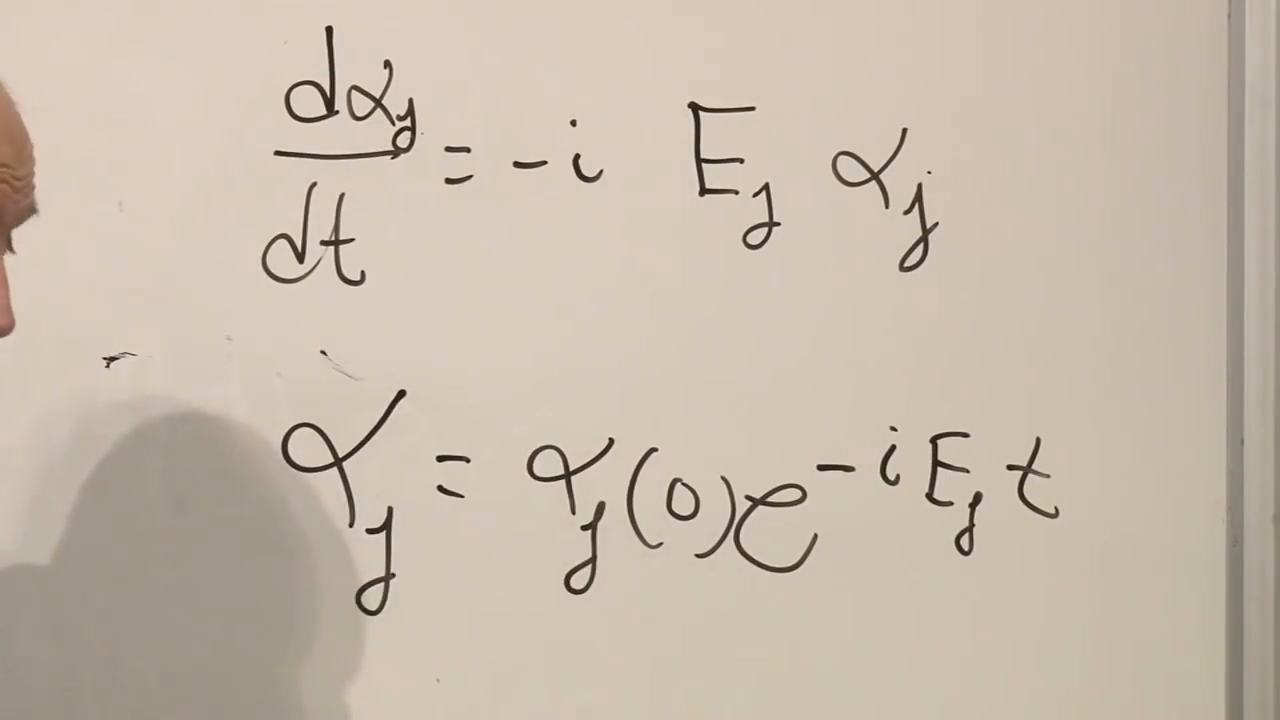
\includegraphics[width=0.86\textwidth]{lecture_05_figure_06.png}
\caption{每个能量基系数都满足自己的指数相位方程。}
\lectureframe{01:03:25}
\end{figure}

因此通解是
\begin{equation}
\ket{\psi(t)}
=\sum_j\alpha_j(0)e^{-iE_jt}\ket{E_j}.
\label{eq:l5-general-solution}
\end{equation}
恢复单位后，\(E_jt\)被替换为\(E_jt/\hbar\)。每个系数的模保持不变：
\begin{equation}
|\alpha_j(t)|=|\alpha_j(0)|.
\end{equation}
时间演化改变相对相位。单个能量本征态只获得一个共同的相位，因此其测量概率与时间无关。

\(L\)的期望值现在可以明确写出。用能量基定义其矩阵元为
\begin{equation}
L_{kj}=\bra{E_k}L\ket{E_j}.
\end{equation}
于是
\begin{align}
\expect{L}(t)
&=\sum_{k,j}
\alpha_k^*(0)\alpha_j(0)
e^{i(E_k-E_j)t}
L_{kj}.
\label{eq:l5-heisenberg-matrix}
\end{align}

\begin{figure}[htbp]
\centering
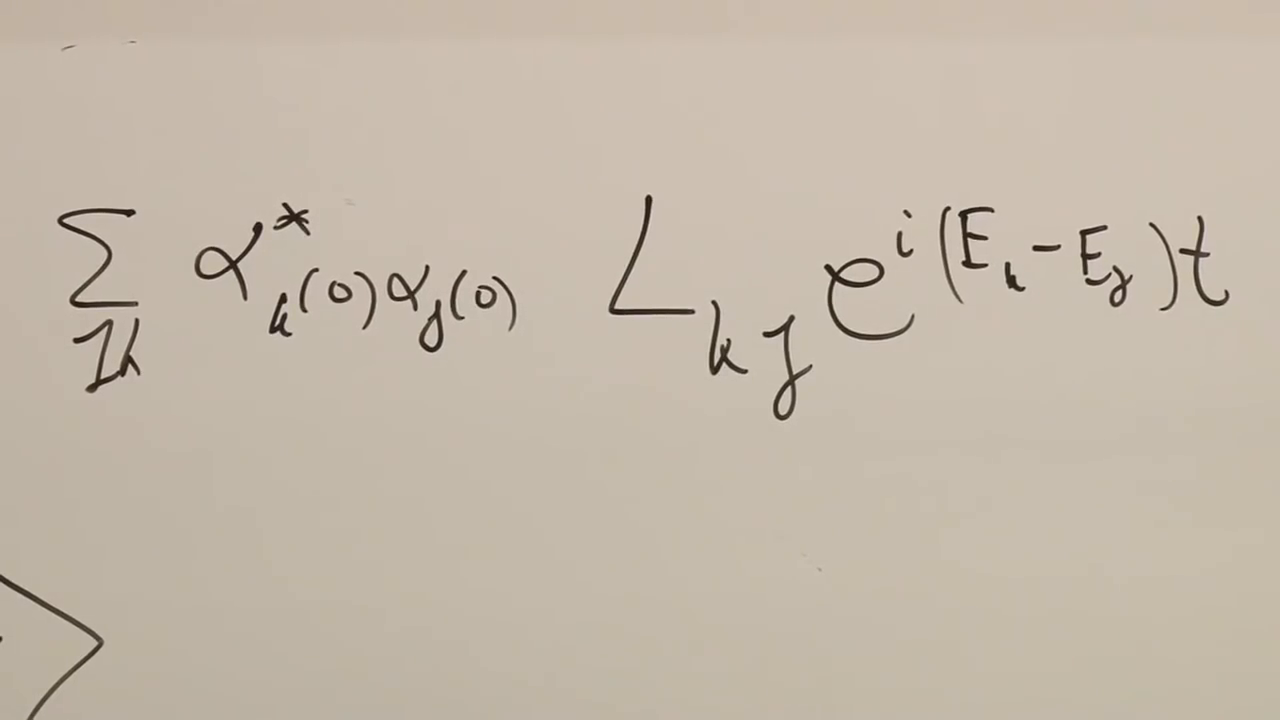
\includegraphics[width=0.86\textwidth]{lecture_05_figure_07.png}
\caption{能量基矩阵公式：每个矩阵元都带有一个跃迁频率的相位。}
\lectureframe{01:10:45}
\end{figure}

对角项\(k=j\)是常数。非对角矩阵元以能量差\(E_k-E_j\)振荡。在这里给出的历史叙述中，海森堡在现代态矢量推导出现之前就认识到了这种矩阵组织方式；狄拉克的记号后来使其含义变得清晰。

\begin{classroomqa}
\audiencequestion{\(\alpha_j\)系数的模是否保持不变？}
\lecturerresponse{是的。每个系数都乘以一个单位模的复相位。只有相对相位改变，而正是这些相位使得含有非对角矩阵元的期望值随时间变化。}
\end{classroomqa}

\begin{classroomqa}
\audiencequestion{Schr\"odinger方程应当使用偏导数还是全导数？}
\lecturerresponse{对于此处所用的抽象态\(\ket{\psi(t)}\)，时间是唯一显含的变量，因此两种记号承载的内容相同。之后，诸如\(\psi(x,t)\)这样的波函数将同时依赖于位置和时间，那时偏导数记号就会显得自然。}
\end{classroomqa}

\begin{classroomqa}
\audiencequestion{正交性的保持仅仅是一个经验假设吗？}
\lecturerresponse{它得到实验支持，但它也异常刚性。试图对幺正量子力学进行形变的尝试往往会破坏正定性或概率守恒、因果局域性，或对复合系统的一致处理。David Finkelstein 将可形变理论描述为发生塑性流动，而将刚性理论描述为脆性开裂。在这个意义上，量子力学是脆性的：任意的小改动通常不会留下一个邻近的一致理论。}
\end{classroomqa}

\begin{classroomqa}
\audiencequestion{为什么能量本征值\(E_j\)是实的？}
\lecturerresponse{幺正性意味着无穷小生成元\(H\)是厄米的，而厄米算符的每个本征值都是实的。因此这一链条是：正交性保持、幺正性、\(H\)的厄米性，以及能量谱的实性。}
\end{classroomqa}

\section{磁场中的一个自旋}

应当为单个自旋赋予什么哈密顿量？一个孤立自旋处于其他方面空无一物的空间中时，没有非平凡的优先方向，因此其哈密顿量正比于单位算符，不产生可观测的运动。磁场则同时提供了相互作用能和一个轴。

取场沿\(z\)方向。带自旋的带电粒子携带磁矩，而熟悉的偶极能量正比于该磁矩与场的对齐程度。将场强、磁矩、符号约定以及\(\hbar\)吸收进一个常数\(\omega\)：
\begin{equation}
H=\frac{\omega}{2}\sigma_z.
\label{eq:l5-z-hamiltonian}
\end{equation}
\(1/2\)这个因子很方便，因为泡利对易子中含有因子\(2\)。

经典的箭头图像必须谨慎处理。量子自旋并不同时具有确定的\(x\)、\(y\)和\(z\)分量，因此没有任何普通箭头能同时表示它的全部性质。有用的三维对象将是期望值矢量，而不是二分量态矢量本身。

\subsection{泡利对易子}

使用矩阵表示
\begin{equation}
\begin{aligned}
\sigma_x&=
\begin{pmatrix}0&1\\1&0\end{pmatrix},\\[0.4em]
\sigma_y&=
\begin{pmatrix}0&-i\\i&0\end{pmatrix},\\[0.4em]
\sigma_z&=
\begin{pmatrix}1&0\\0&-1\end{pmatrix}.
\end{aligned}
\end{equation}
例如，
\begin{align}
[\sigma_z,\sigma_x]
&=
\begin{pmatrix}1&0\\0&-1\end{pmatrix}
\begin{pmatrix}0&1\\1&0\end{pmatrix}
-
\begin{pmatrix}0&1\\1&0\end{pmatrix}
\begin{pmatrix}1&0\\0&-1\end{pmatrix}\\
&=
\begin{pmatrix}0&1\\-1&0\end{pmatrix}
-
\begin{pmatrix}0&-1\\1&0\end{pmatrix}\\
&=2
\begin{pmatrix}0&1\\-1&0\end{pmatrix}
=2i\sigma_y.
\end{align}
循环关系为
\begin{equation}
\begin{aligned}
[\sigma_z,\sigma_x]&=2i\sigma_y,\\
[\sigma_x,\sigma_y]&=2i\sigma_z,\\
[\sigma_y,\sigma_z]&=2i\sigma_x.
\end{aligned}
\label{eq:l5-pauli-commutators}
\end{equation}
交换任一位置都会使符号反转。

\begin{figure}[htbp]
\centering
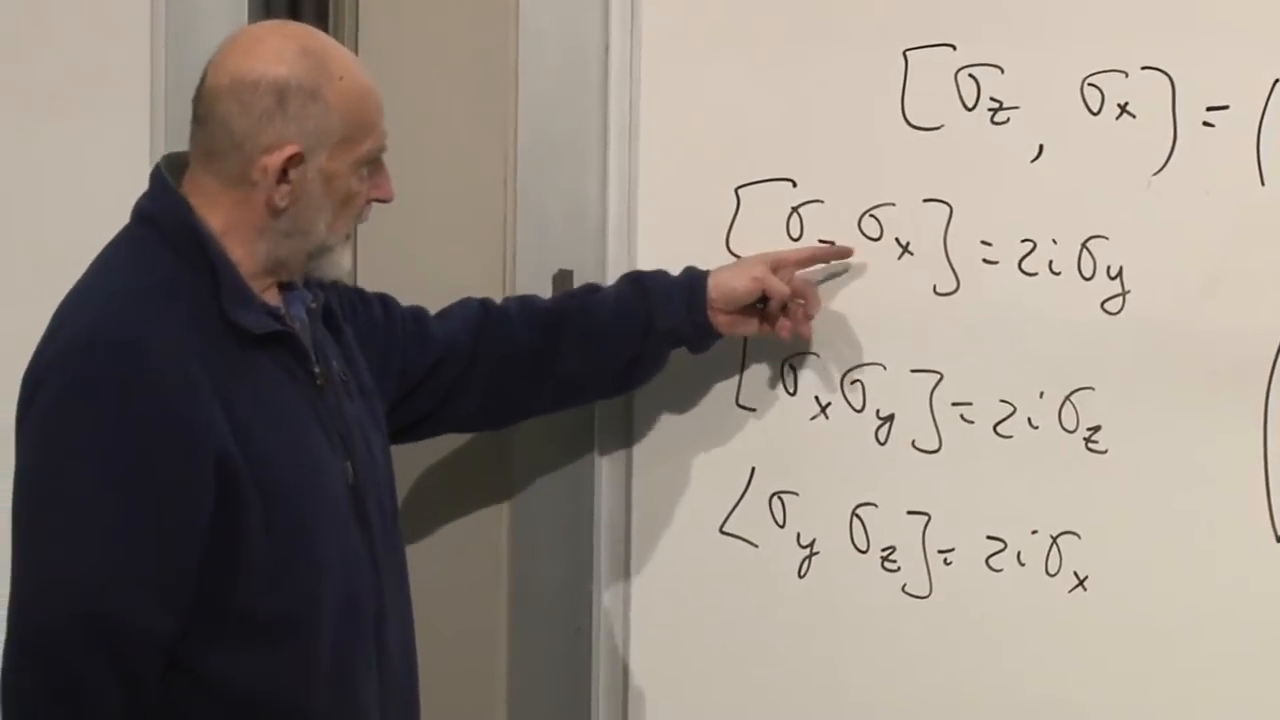
\includegraphics[width=0.86\textwidth]{lecture_05_figure_08.png}
\caption{三个泡利对易子以循环方式在泡利矩阵自身之上封闭。}
\lectureframe{01:33:30}
\end{figure}

这些关系与角动量的经典泊松括号具有相同的循环结构。它们也在原来的三个算符之上封闭，这使得运动方程特别简单。

\begin{classroomqa}
\audiencequestion{对易子必须用左右矢括号来计算吗？}
\lecturerresponse{不。算符乘法由矩阵乘法表示，因此\(2\times2\)矩阵提供了一种方便的直接计算。也可以改为将算符依次作用于自旋上和自旋下的基态，得到相同结果。}
\end{classroomqa}

\subsection{期望值的进动}

将方程~\eqref{eq:l5-expectation-motion}与方程~\eqref{eq:l5-z-hamiltonian}中的哈密顿量一起应用：
\begin{align}
\frac{d}{dt}\expect{\sigma_x}
&=-i\frac{\omega}{2}\expect{[\sigma_x,\sigma_z]}
=-\omega\expect{\sigma_y},\\
\frac{d}{dt}\expect{\sigma_y}
&=-i\frac{\omega}{2}\expect{[\sigma_y,\sigma_z]}
=+\omega\expect{\sigma_x},\\
\frac{d}{dt}\expect{\sigma_z}
&=-i\frac{\omega}{2}\expect{[\sigma_z,\sigma_z]}
=0.
\label{eq:l5-spin-motion}
\end{align}

\begin{figure}[htbp]
\centering
\begin{minipage}[c]{0.62\textwidth}
\centering
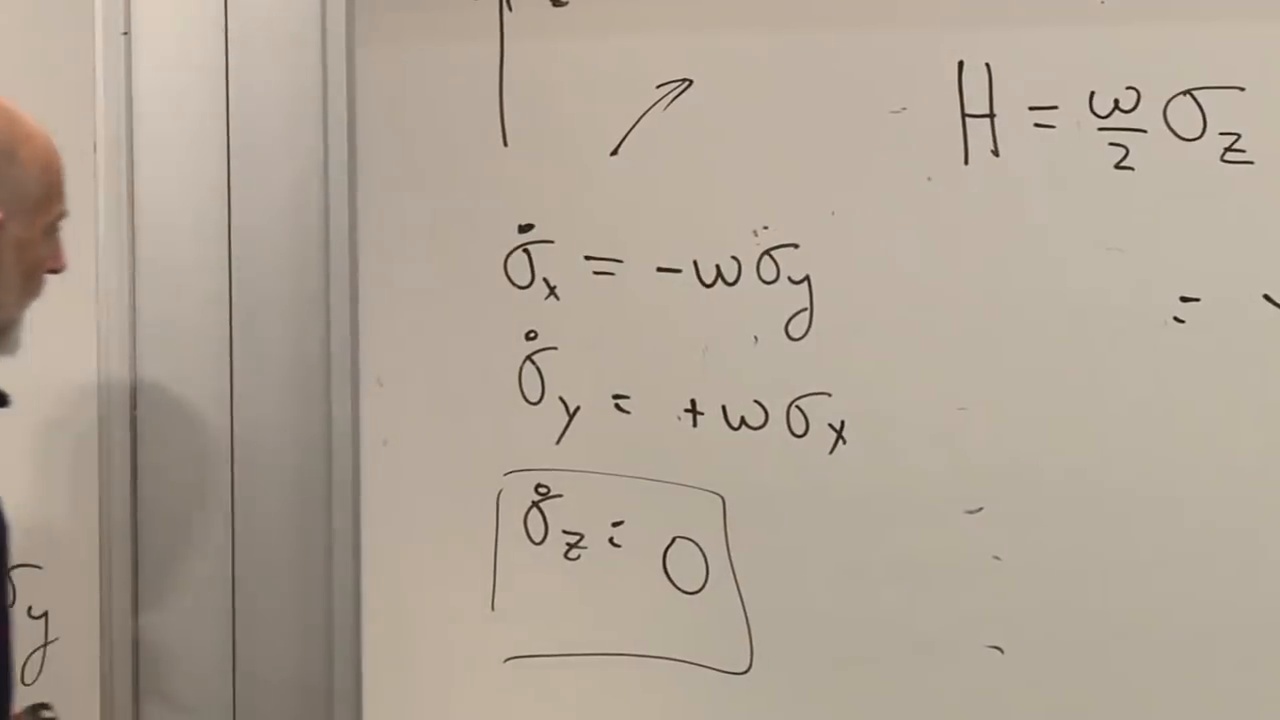
\includegraphics[width=\textwidth]{lecture_05_figure_09.png}
\end{minipage}\hfill
\begin{minipage}[c]{0.31\textwidth}
\centering
\begin{tikzpicture}[scale=0.78,>=Latex]
  \draw[->,thick] (0,0) -- (0,3.0) node[above] {\(z\parallel\bm B\)};
  \draw[dashed] (0,1.8) ellipse (1.45 and 0.42);
  \draw[->,very thick] (0,0) -- (1.05,1.8)
    node[right] {\(\expect{\bm\sigma}\)};
  \draw[->,thick] (1.38,1.67)
    arc[start angle=-12,end angle=245,x radius=1.45,y radius=0.42];
\end{tikzpicture}
\end{minipage}
\caption{板书方程及其几何推论：横向平均值旋转，而平行于场的分量保持不变。箭头描绘的是三个期望值，而不是隐藏的经典自旋。}
\lectureframe{01:35:28}
\end{figure}

前两个方程描述横向平面中的圆周运动：
\begin{align}
\expect{\sigma_x}(t)
&=\expect{\sigma_x}(0)\cos\omega t
-\expect{\sigma_y}(0)\sin\omega t,\\
\expect{\sigma_y}(t)
&=\expect{\sigma_x}(0)\sin\omega t
+\expect{\sigma_y}(0)\cos\omega t.
\end{align}
与此同时\(\expect{\sigma_z}\)是常数。因此期望值矢量以角频率\(\omega\)绕磁场轴进动。

在这个Schr\"odinger绘景中，算符是固定矩阵。变化的是态，因而执行熟悉的陀螺运动的是平均值。

\begin{classroomqa}
\audiencequestion{二维态空间如何能产生三维的进动图像？}
\lecturerresponse{态矢量有两个复分量，在归一化和整体相位意义下如此。而所绘制的实空间矢量则是\(\bigl(\expect{\sigma_x},\expect{\sigma_y},\expect{\sigma_z}\bigr)\)。这些期望值由态决定，并构成布洛赫矢量图像，但它们并不是态矢量本身。}
\end{classroomqa}

\section{最一般的单自旋哈密顿量}

每个厄米\(2\times2\)矩阵都可以展开为
\begin{equation}
H=aI+b_x\sigma_x+b_y\sigma_y+b_z\sigma_z,
\end{equation}
其中系数为实数。单位项只改变整体相位。其余三个系数可以看作一个矢量的分量。将其大小记为\(\omega/2\)，方向记为单位矢量\(\bm n\)，则非平凡哈密顿量变为
\begin{equation}
H=\frac{\omega}{2}\,\bm\sigma\cdot\bm n,
\qquad
\bm\sigma\cdot\bm n
=n_x\sigma_x+n_y\sigma_y+n_z\sigma_z.
\label{eq:l5-general-spin-h}
\end{equation}
若\(\bm B=B\bm n\)，则\(\bm n\)携带场的方向，而\(\omega\)连同磁耦合一起携带场的大小。记录取向的是\(\bm n\)，而不是\(\omega\)。

运动方程取紧凑形式
\begin{equation}
\frac{d}{dt}\expect{\bm\sigma}
=\omega\,\bm n\times\expect{\bm\sigma}.
\end{equation}
沿\(\bm n\)的分量与\(H\)对易并保持固定；垂直分量绕\(\bm n\)进动。

\begin{classroomqa}
\audiencequestion{为什么这是哈密顿量的正确形式？}
\lecturerresponse{独立的厄米\(2\times2\)矩阵只有四个：\(I,\sigma_x,\sigma_y,\sigma_z\)。单位矩阵不贡献任何可观测的单自旋运动，因此每个非平凡的时间无关单自旋哈密顿量都是三个泡利矩阵的实线性组合。磁场将这三个系数打包成大小和方向。}
\end{classroomqa}

\begin{classroomqa}
\audiencequestion{\(\omega\)究竟代表什么？}
\lecturerresponse{它是一个标量，正比于场的大小乘以磁矩，常规常数已吸收其中。它同时决定进动速率和能级分裂。单位矢量\(\bm n\)指定场的方向。}
\end{classroomqa}

\subsection{两个能级}

将方程~\eqref{eq:l5-general-spin-h}写成矩阵，得到
\begin{equation}
\bm\sigma\cdot\bm n
=
\begin{pmatrix}
n_z & n_x-in_y\\
n_x+in_y & -n_z
\end{pmatrix}.
\end{equation}
设其本征值为\(\lambda_1,\lambda_2\)。其迹为零：
\begin{equation}
\lambda_1+\lambda_2=0.
\end{equation}
对于单位矢量\(n_x^2+n_y^2+n_z^2=1\)，其行列式为
\begin{align}
\lambda_1\lambda_2
&=\det(\bm\sigma\cdot\bm n)\\
&=-n_z^2-(n_x-in_y)(n_x+in_y)\\
&=-(n_x^2+n_y^2+n_z^2)\\
&=-1.
\end{align}
因此两个本征值为
\begin{equation}
\lambda_\pm=\pm1.
\end{equation}

\begin{figure}[htbp]
\centering
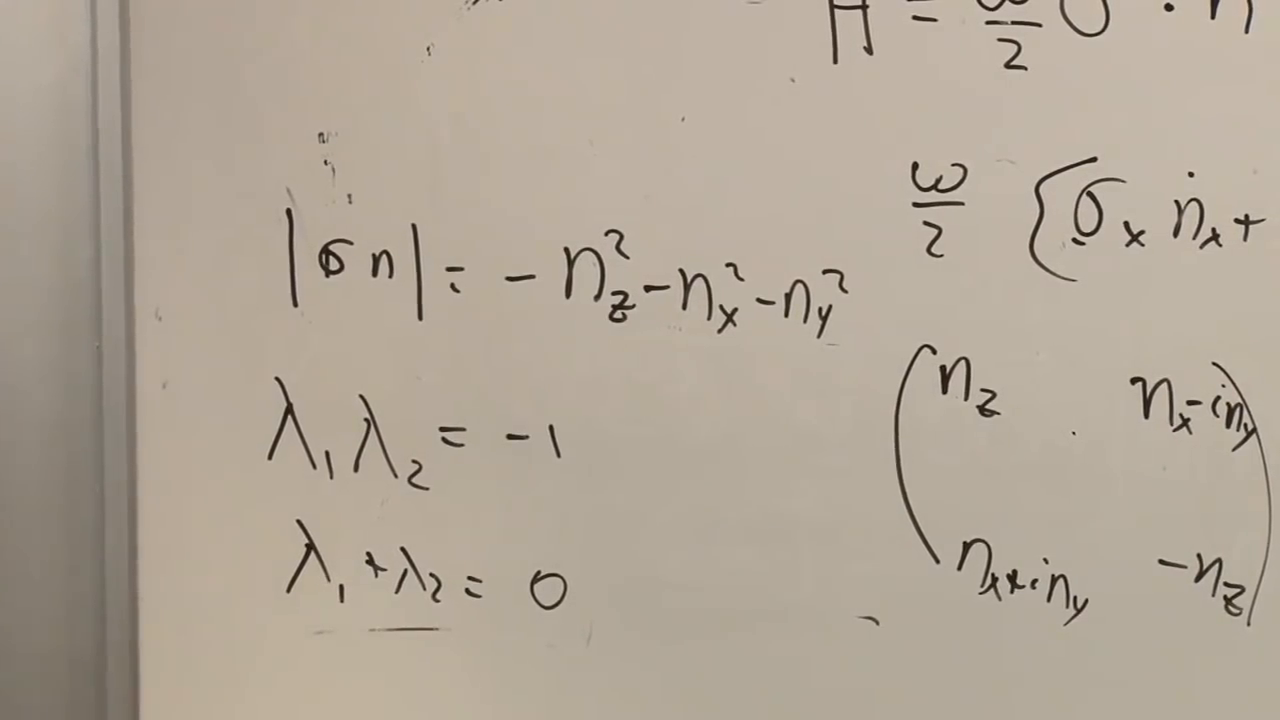
\includegraphics[width=0.86\textwidth]{lecture_05_figure_10.png}
\caption{迹和行列式将\(\bm\sigma\cdot\bm n\)的本征值确定为\(+1\)和\(-1\)。}
\lectureframe{01:59:20}
\end{figure}

因此，
\begin{equation}
E_\pm=\pm\frac{\omega}{2},
\qquad
\Delta E=E_+-E_-=\omega.
\label{eq:l5-spin-gap}
\end{equation}
场的方向改变能量本征矢量，但不改变这两个本征值。

\begin{classroomqa}
\audiencequestion{光子发射与这些能级有什么关系？}
\lecturerresponse{将辐射场包括在内时，较高的自旋能级可以通过发射一个能量为\(\Delta E=\omega\)的光子衰变到较低能级，这里采用当前的\(\hbar=1\)约定。自旋随后在沿场轴的两个相反取向之间翻转。进动计算忽略了这一微弱辐射耦合，因此自旋在发射之前可以进动许多次。}
\end{classroomqa}

\begin{classroomqa}
\audiencequestion{为什么磁场被当作数而不是量子算符处理？}
\lecturerresponse{磁体暂时被当作一个重的经典仪器，其涨落和反冲可以忽略。完整的描述会把它包括在一个更大的量子系统中。当仪器具有许多自由度，并且其相关变量的涨落小到电子无法明显改变它们时，实际中的系统-仪器划分就是合理的。}
\end{classroomqa}

\begin{classroomqa}
\audiencequestion{光滑的进动方程描述每一次单独试验吗？}
\lecturerresponse{它们描述期望值，因此是对相同制备试验的平均。单次测量仍然是概率性的。重复样本倾向于近似理论平均值，但概率论并不保证每个有限序列都有一个精确结果，正如一百万次抛硬币不必恰好包含一半正面。}
\end{classroomqa}

\begin{classroomqa}
\audiencequestion{如果自旋指向侧面，跃迁会发射半个光子吗？}
\lecturerresponse{不会。侧向自旋态是两个能量本征态的叠加。在对称情形下，它处于上能级的概率为一半，处于下能级的概率也为一半。因此它可能发射一个能量为\(\omega\)的完整光子，也可能不发射。其平均发射能量可以是\(\omega/2\)，但没有单个光子携带能级间距的一半。}
\end{classroomqa}

我们现在已经穷尽了单个自旋的非平凡时间无关动力学。最初预示不确定性的同一套代数也生成了它的运动：不对易的泡利矩阵将哈密顿量变成进动，而与哈密顿量对易的分量保持守恒。复杂性的下一次增加不是另一个单自旋哈密顿量，而是更大的态空间，在那里独立的系统可以被组合和纠缠。
